\documentclass[progress]{cmpreport}
\graphicspath{ {./images/} }

\title{GPU Accelerated Method for Constructing and Rendering Trees 
        \\ - \\ 
        Progress Report}
\author{Thomas Mcloughlin}
\date{3/12/2020}
\registration{100203952}
\ccode{CMP - 6013Y}
\supervisor{Dr. Stephen Laycock}

\begin{document}
\maketitle

\section{Description of the Project}
This section will outline the aims and motivation of the project, describing why this system 
would be useful in a 3D graphics environment application.

\subsection{Aims}
The aim of this project is to produce an OpenGL module for constructing and rendering trees 
that can be placed in a 3D environment. These trees should be randomly generated to allow 
for multiple trees to be rendered and not have them look the same. They should use a suitable 
algorithm to produce this randomness that will control the structure of branches and leaf 
placement on those branches.

\subsection{Motivation}
The motivation for producing this system is to reduce the effort that needs to be dedicated to 
creating a realistic looking 3D environment. Simulating nature can be difficult and that is 
shown in the construction of trees and other foliage. Having a designer create each tree model 
from scratch while trying to make each model look realistic and varied would be a huge 
undertaking and take a long time. Whereas using this system would allow for quick and easy 
construction and placement of trees in an environment, with user input allowing for certain 
aspects of the generated trees to be tweaked to the required specifications.

\section{Description and Understanding of Issues and Problems}
In this section the various issues and problems that have arisen during the design stage of the 
project will be listed and explained.

\subsection{Branch Structure}
The choice of what method to use for branch structure when approaching this project is the 
issue which will have the largest affect on the result. Different algorithms are likely to 
produce different results in the final branch structure so care was put in to understand the 
various methods and choose one that would be most suitable with a balance between attaining a 
realistic looking result and ease of implementation.

The choices were separated between methods described in various papers found as part of the 
Literature Review and after much consideration the decision was made to use L-systems, 
described by \cite{prusinkiewicz1996systems}, to create the branch structure in the trees. 
This would be done by creating preset constructed parts to act as our variables, using a chosen 
point in the environment as an axiom and providing the rules to construct the tree geometry. 
Some variation at each level needs to be applied to give a sense of natural growth, this would 
include a variation in branching angle each time a branch splits off from the previous branch. 
The user control can be presented through the rules of the L-system, by changing these rules 
the user could affect how the tree is constructed.

\subsection{Leaf Placement}
The problem with leaf placement is having the system decide where will be appropriate to place 
leaves to make the tree realistic looking. \cite{prusinkiewicz1996systems} combine leaf 
placement with the construction of the branches, where some variables in the chosen L-system 
include adding leaves to the constructed branch or having a terminating branch end in a leaf. 
This is decidedly too basic for use with a more detailed 3D application and so this idea will 
be combined with a method presented by \cite{weber1995rendering} where leaf placement can be 
decided based on the level of a branch. The level being the number of parental branches that 
the current branch has meaning the more parents the branch has usually means that the branch 
is further from the trunk and more likely to be a terminating branch. Leaf placement will be 
done only on branches of a certain level and above to give the trees the proper dispersion of 
leaves across outwards reaching branches.

The issue of how specifically to add leaves to the chosen branches requires another method. 
\cite{weber1995rendering} do describe their method for leaf placement somewhat but only 
give a formula for deciding the number of leaves to be placed and not specifically how they 
are placed. For this a method of random placement needs to be inferred and the chosen method 
involves these steps: decide the number of leaves needed for a chosen branch, choose varying 
points along the branch where the leaves will be placed, render the leaves, orient the leaves 
semi-randomly while taking into account the position of the tree.

\section{Design and Planning}
As a simulation project this design plan will give a design of the chosen simulation model 
supported by example pseudo code and diagrams.


The chosen simulation model for this project is the use of L-systems which has been loosely 
explained but will be described in more detail here.

A Lindenmayer system (L-system) is a system of ordering an alphabet of symbols to make 
strings. The symbols are formed into the string using production rules that expand each 
symbol into some larger string of symbols. The expansion starts from an initial axiom string 
which is some chosen collection of symbols, changing the axiom string is a way to alter the 
resulting string without changing any of the symbols or rules involved in the system. The 
number of times you apply the rules to the string (number of recursions) will also give you 
different strings, and a chosen recursion depth may be chosen to give a desired affect.\\

Below is an example of a very basic L-system which can model a fractal tree:\\

\noindent \textbf{variables:} 0, 1 \\
\textbf{constants:} [, ] \\
\textbf{axiom:} 0 \\
\textbf{rules:} (1 $\rightarrow$ 11), (0 $\rightarrow$ 1[0]0) \\

which will produce: \\

\noindent \textbf{axiom:} 0 \\
\textbf{1st recursion:} 1[0]0 \\
\textbf{2nd recursion:} 11[1[0]0]1[0]0 \\
\textbf{3rd recursion:} 1111[11[1[0]0]1[0]0]11[1[0]0]1[0]0 \\

\pagebreak
If we take each variable from this string and apply a graphics drawing command to each 
variable to construct a tree by traversing the string left to right using the commands below: \\

\noindent \textbf{0:} draw a line segment ending in a leaf \\
\textbf{1:} draw a line segment \\
\textbf{[:} push position and angle, turn left 45 degrees \\
\textbf{]:} pop position and angle, turn right 45 degrees \\

This example uses turtle graphics as an example due to the simplicity of the L-system but this 
same method could be applied to 3D graphics with a more complex set of system variables.\\

\begin{figure}[h]
        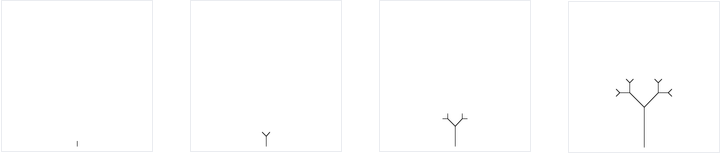
\includegraphics[scale=0.75]{l-system}
        \caption{The axiom and results of the first 3 recursions of the example L-system}
        \centering
\end{figure}

\clearpage
\bibliography{bibfile}
\end{document}